\section{State of the art}

The contemporary secure communication protocols such as TLS, OpenVPN, and IPSec utilizes the following structure: 
\begin{figure}[H]
    \centering
    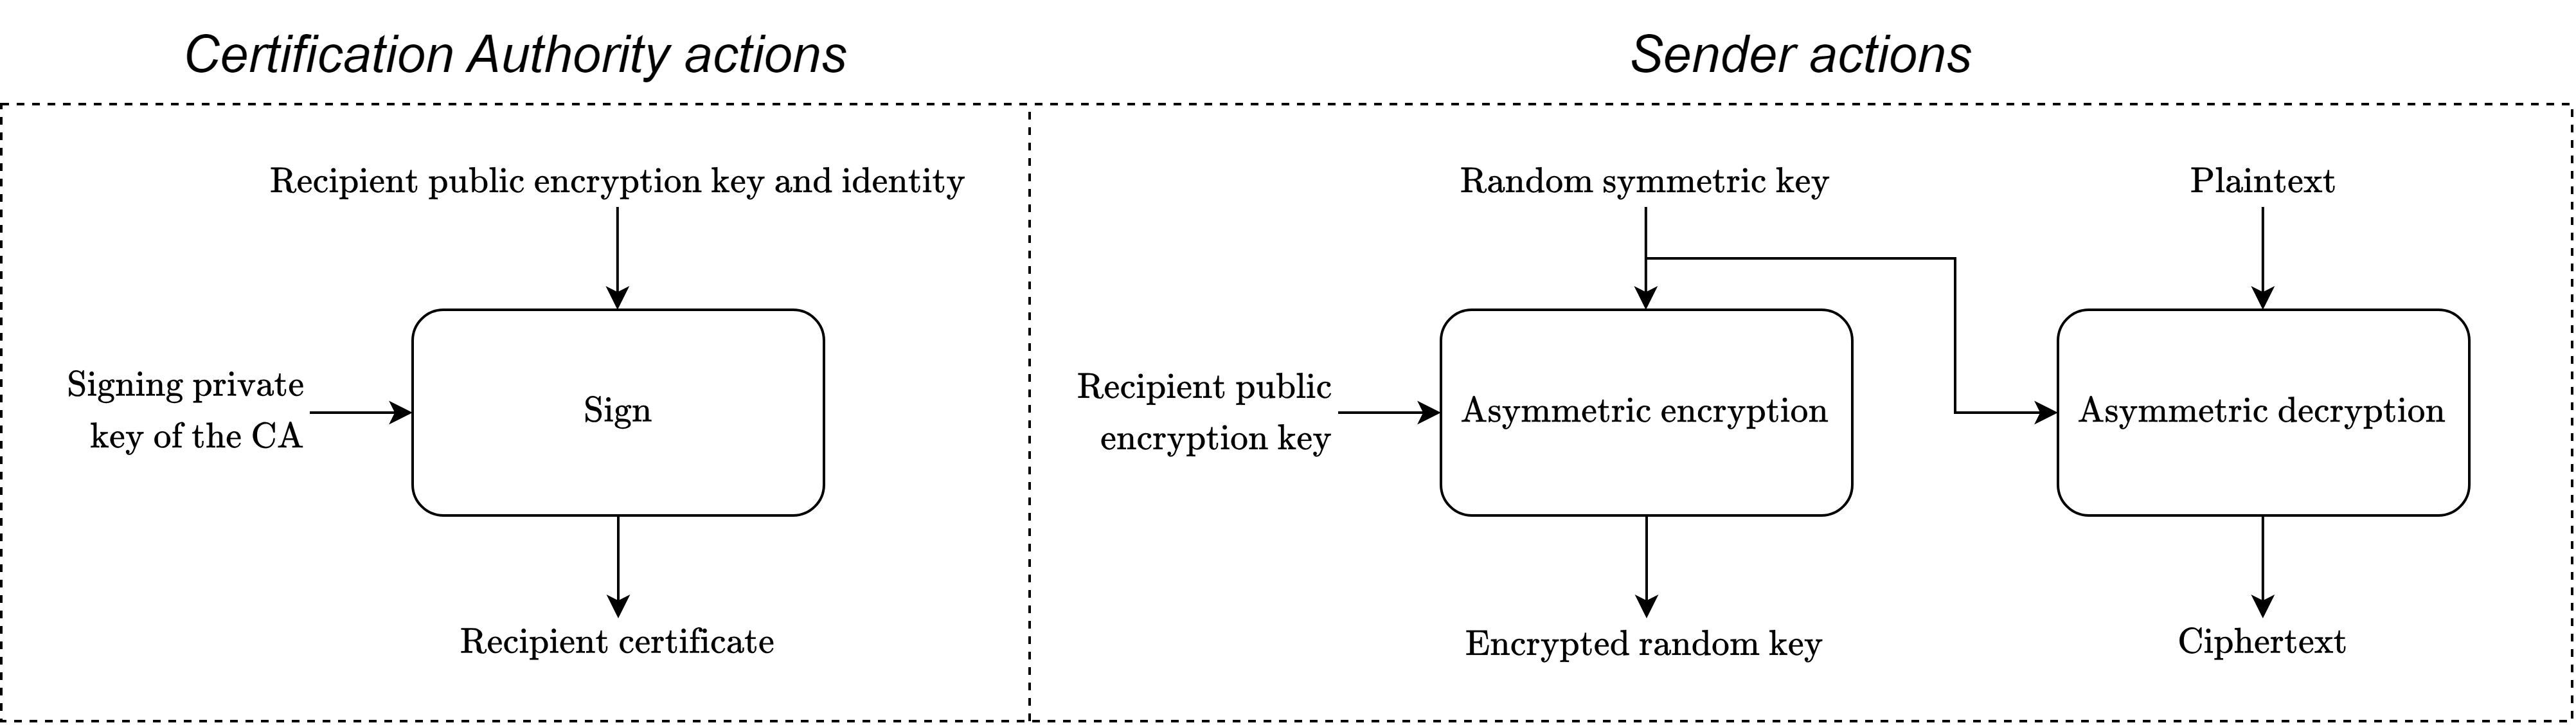
\includegraphics[width=1\linewidth]{images/ssp.png}
    \caption{Secure communication protocols}
\end{figure}

\paragraph*{Quantum computers}
With quantum computing some computationally challenging problems will become less hard, prompting a reassessment of their difficulty. 
There's a notable shift away from cryptosystems built upon factoring and discrete logarithm. 
Instead, there's a growing focus on exploring alternatives, currently undergoing standardization as of April 2022.

\paragraph*{Compute on encrypted data}
Performing computations on encrypted data is feasible; however, it tends to be moderately to severely inefficient.

\paragraph*{Physical access}
If the attacker gains physical access to the device executing the cipher (or can remotely measure it), it is essential to consider side-channel information within the attacker model.